\chapter{Hardware}

Im Kapitel 5 wird die verwendete Hardware vorgestellt. Dies sind der Lidar, der Einplatinencomputer Raspberry Pi 3b+ sowie das Interface Board mit seinen angschlossenen Sensoren. 

\section{Lidar}

Als Laserscanner wird ein Hokuyo URG-04LX verwendet.

Dieser hat eine Auflösung von 360° / 1024 pro Step. Insgesamt kann ein Winkel von 240° (= 768 Datenpunkte) je Scan aufgezeichnet werden.

\begin{figure}[h]
\begin{center}
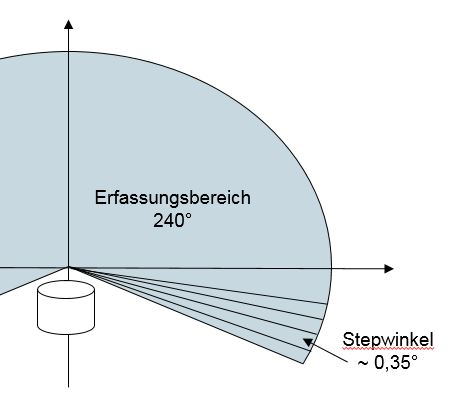
\includegraphics[width=10cm]{images/chapter5/LidarHardware.jpg}
\caption{Lidar Uebersicht}
\label{Lidar_uebersicht}
\end{center}
\end{figure}

Die Daten werden für jeden erfassten Punkt jeweils im Abstand von 0,35° als Entfernung geliefert. Die Punkte sind somit in Polarkoordinaten Darstellung vorhanden \cite{hokuyo.2018}.

\begin{figure}[h]
\begin{center}
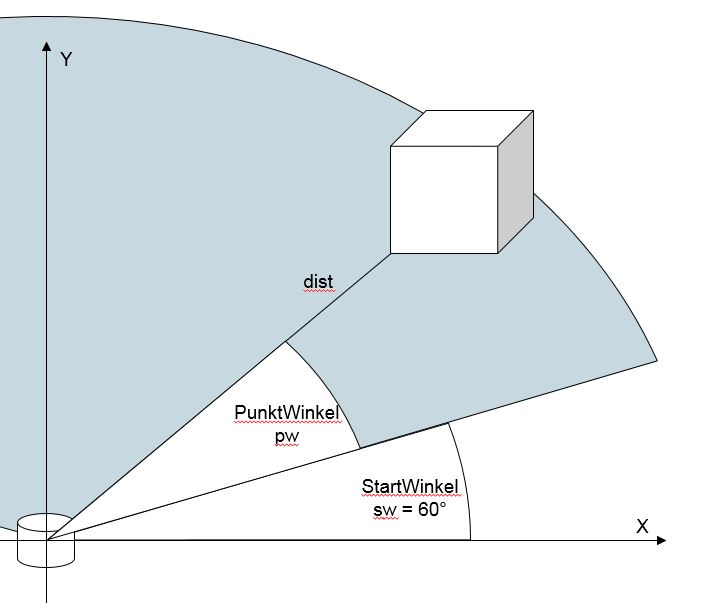
\includegraphics[width=10cm]{images/chapter5/LidarWinkeluebersicht.jpg}
\caption{Lidar Uebersicht}
\label{Lidar_uebersicht}
\end{center}
\end{figure}

\section{Raspberry Pi 3b+}

Als Hauptrechner wurde sich für den Raspberry Pi 3b+ der aktuellsten Generation entschieden. Aufgrund seiner ausreichenden Leistung von 4 Kernen mit je 1.4 GHz und mit einem Arbeitsspeicher von 1 GB werden auf diesem Rechner der Slam sowie die Wegefindung ausgeführt. Außerdem bietet dieser noch ausreichend Kapaziät für Erweiterungen in der Software und Hardware durch nachfolgende Gruppen.  


\begin{figure}[hbtp]
\centering
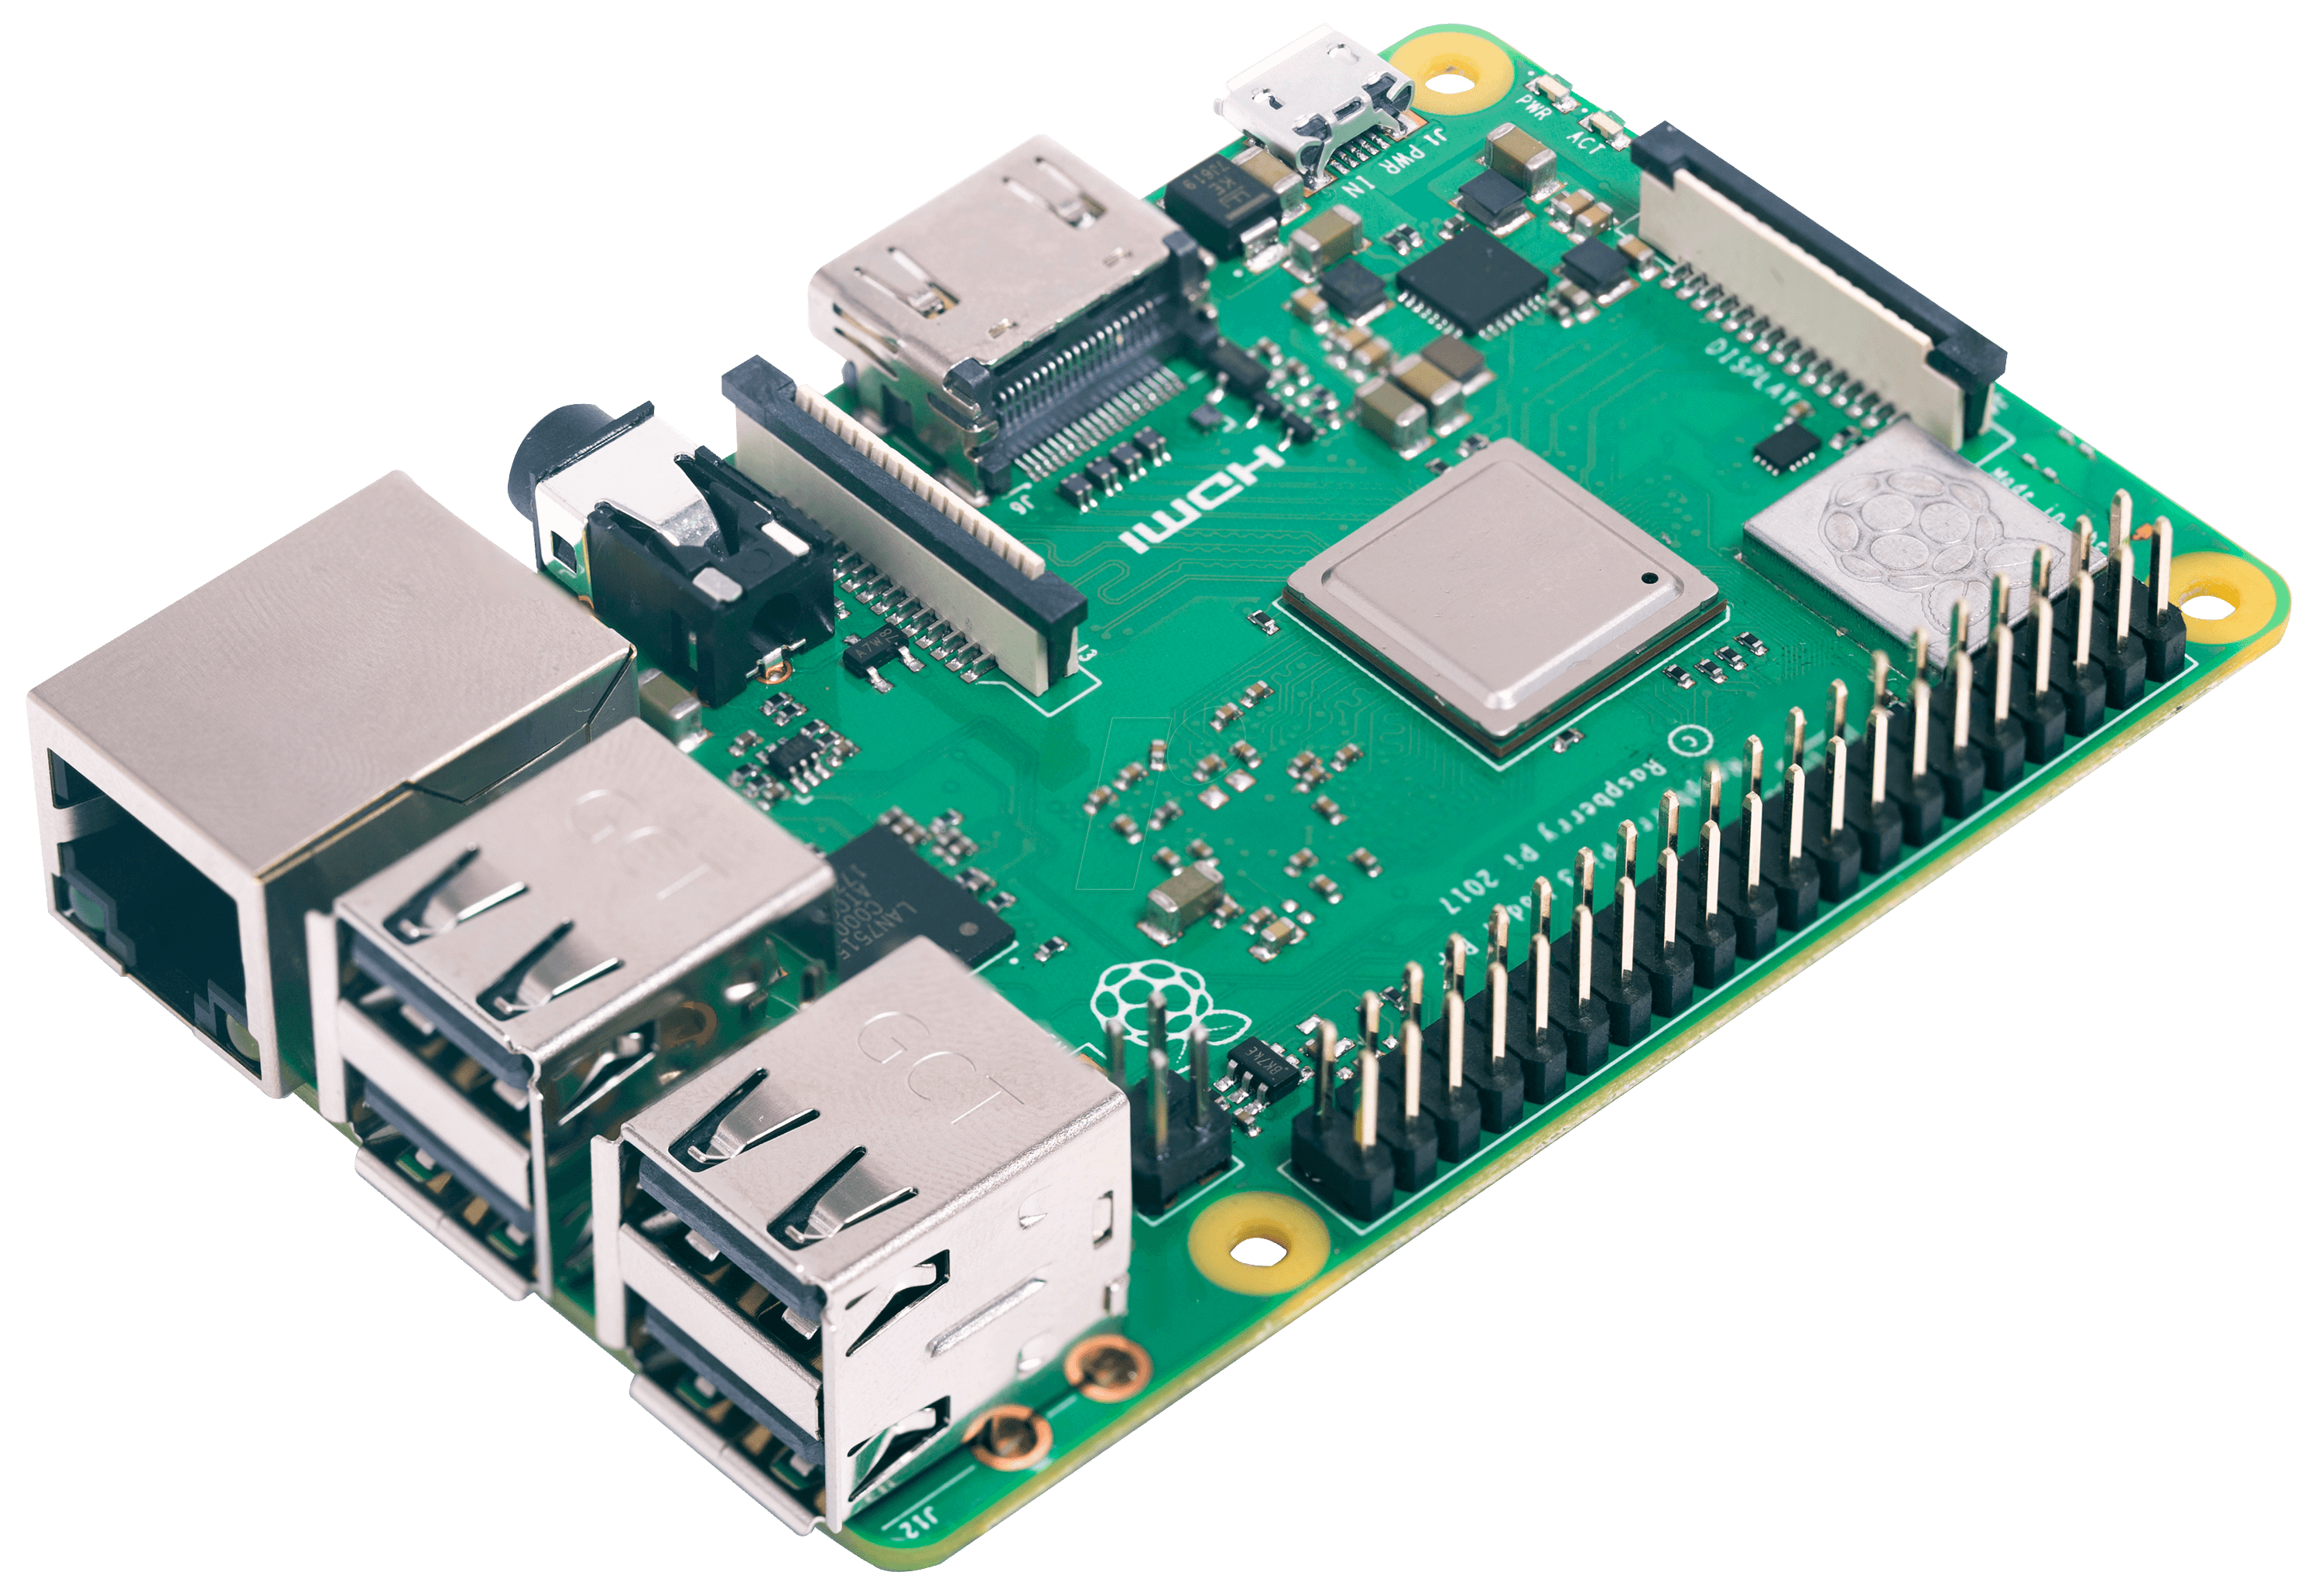
\includegraphics[scale=0.1]{images/chapter5/raspberry.png}
\caption{Der Raspberry Pi 3b+ \cite{raspberry.2018}}
\label{fig:raspberry}
\end{figure}






\newpage
\section{Interface Board}
\label{sec:InterfaceBoard}
\subsection{Konzept und Aufbau}

Um die verwendeten Sensoren und Aktuatoren in einer deterministischen Zeit kontrollieren und auslesen zu können, wurde neben dem Raspberry Pi 3B+ Board ein zweites Hardwaremodul verwendet. Es handelt sich hierbei um ein \textit{STM32 F334R8 Nucleo Board} der Firma STMicroelectronics \footnote{www.st.com}. Auf dem Board befindet sich ein ARM Cortex M4 Microcontroller, der für beliebige Mess- und Regelungsaufgaben programmiert werden kann. Folgen Vorteile und Eigenschaften bietet das eingesetzte Board:
\begin{itemize}
\item ARM Cortex - M4 Controller mit 64 MHz und 64 kByte Flash
\item Arduino$^{\textregistered}$ kompatibler Erweiterungssteckplatz
\item viele 3.3V I/Os, einige davon 5V tolerant
\item OnBoard ST-LINK$^{\textregistered}$ V2 Debugger
\end{itemize}

Abbildung \ref{pic:STM32NucleoBoardPicture} zeigt das verwendete Board in der Übersicht.

\begin{figure}[hbtp]
\centering
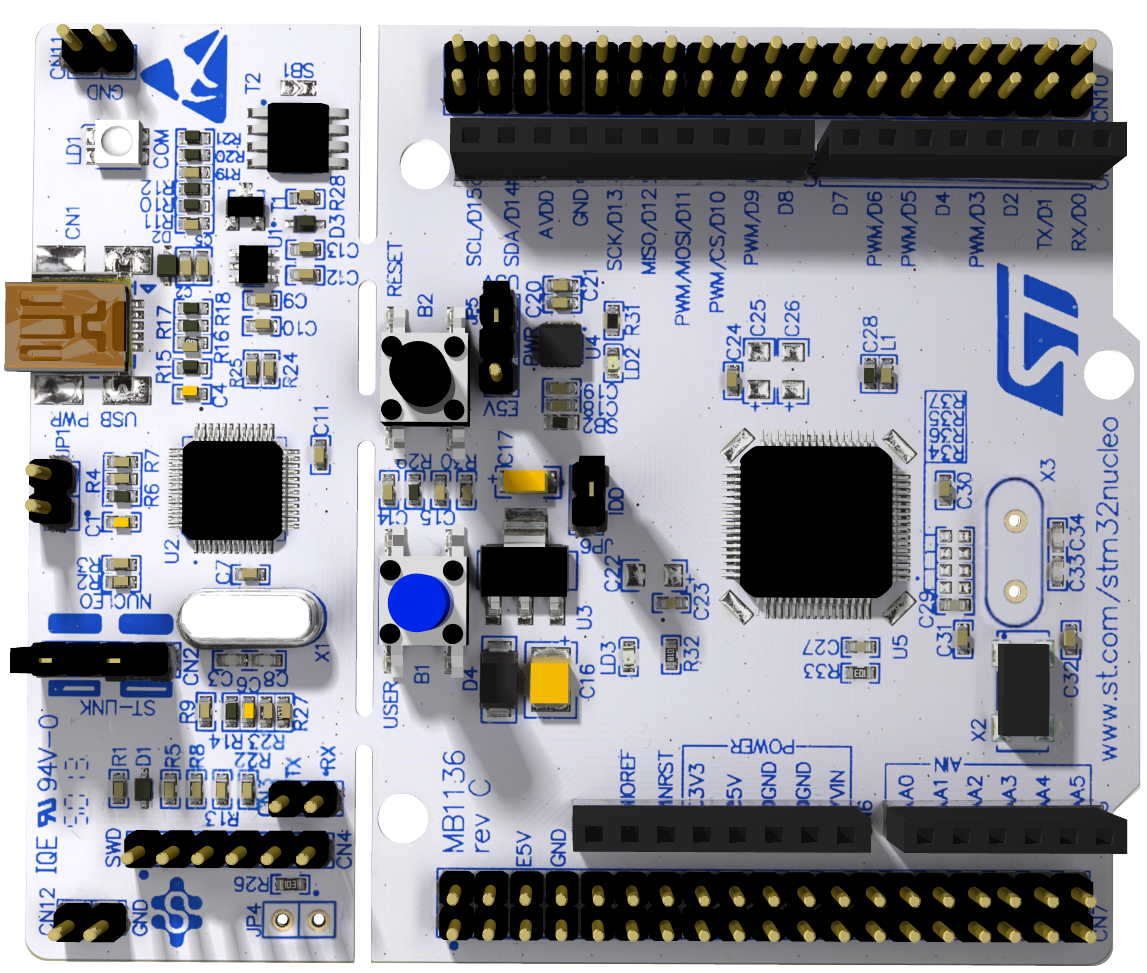
\includegraphics[scale=0.4]{images/chapter5/STMNucleoBoardPicture.png}
\caption{Verwendetes STM32 Nucleo Board Übersicht}
\label{pic:STM32NucleoBoardPicture}
\end{figure}


Zusätzlich verfügt das ALF über folgende Komponenten:
\begin{itemize}
\item 1 Fahrmotor
\item 1 Servo für die Lenkung
\item 3 Ultraschallsensoren (verbunden über I$^{2}$C)
\item 1 kombinierter Beschleunigungssensor und Gyroskop (IMU MPU6050, verbunden über I$^{2}$C)
\end{itemize}

Die Aufgaben des Boards lauten demnach wie folgt:
\begin{itemize}
\item Auslesen der 3 Ultraschall Sensoren (SRF08 Module) im 75ms Takt (I$^{2}$C)
\item Auslesen des Beschleunigungssensors und Gyroskops MPU6050 im 50ms Takt (I$^{2}$C)
\item Kommunikation mit der Hauptrechnerplatine Raspberry Pi über SPI (DMA)
\item Steuerung des Servomotors für die Lenkung (PWM)
\item Steuerung der Richtung und Geschwindigkeit des Fahrmotors (GPIO, PWM)
\end{itemize}
Das Bild \ref{fig:IfBoardHWUebersicht} zeigt die grobe Übersicht über die momentane Hardwarearchitektur des Interface Boards in Kombination mit dem Raspberry Pi. Über die Erweiterungsschnittstelle des STM Boards wurde zudem die Stromversorgung realisiert. Die Akkuspannung (Nennwert 7.2V) wird von einem Step-Down Reglermodul auf die Spannung von 5V konvertiert. Die 5V Logikspannung wird dann an das STM32 Board selbst, an die angeschlossenen Sensoren, und den Raspberry Pi verteilt.

\begin{figure}[hbtp]
\centering
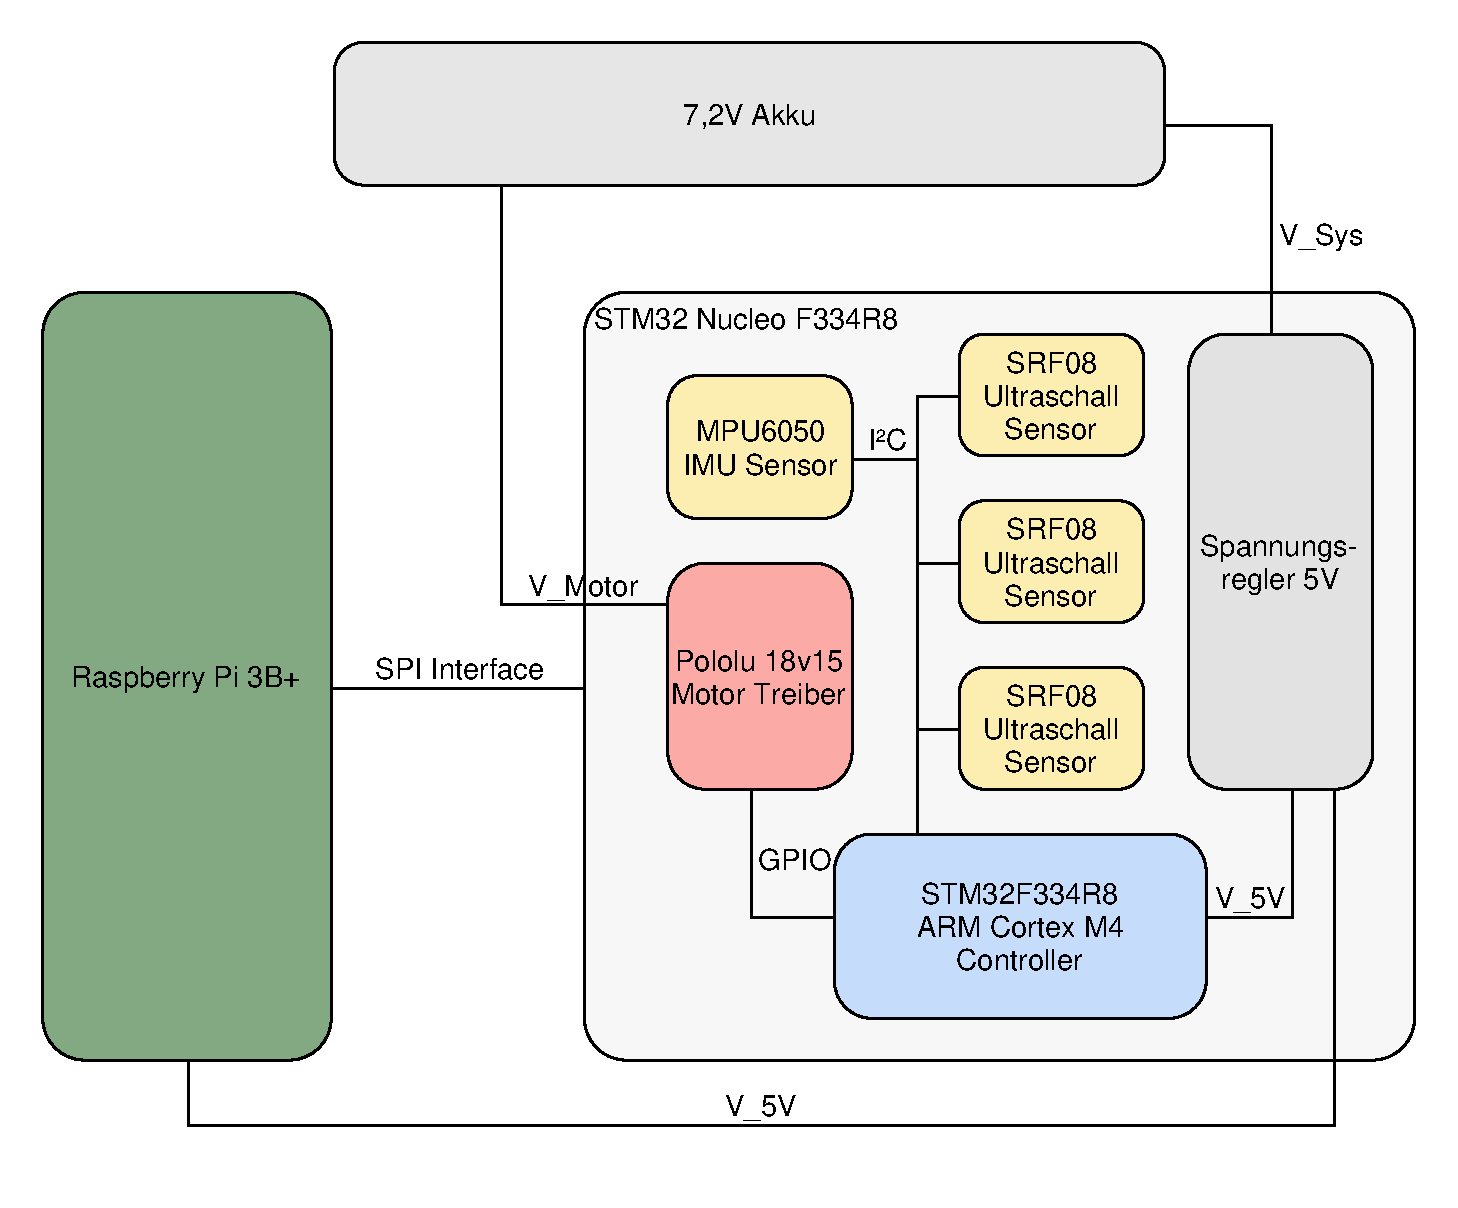
\includegraphics[scale=0.5]{images/chapter5/HW-Architecture.pdf}
\caption{Aktuelle Hardware Architektur des ALF \label{fig:IfBoardHWUebersicht}}
\end{figure}

\subsection{Datenübertragung}

Zwischen dem Interface Board und dem Raspberry Pi findet ein regelmäßiger Datenaustausch statt. Dieser soll den Programmablauf der Firmware auf dem STM32 Controller möglichst nicht unterbrechen, um Echtzeitverhalten sicherzustellen. Deshalb wurde bei der Datenübertragung auf die DMA Hardware des STM32 Controllers zurückgegriffen. Bei jedem Datentransfer, der vom Raspberry Pi (SPI Master) zum Interface Board (SPI Slave) erfolgt, ist die Unterbrechungsdauer des ARM Prozessors auf dem Interface Board so auf einem Minimum reduziert. Die Daten werden in einen definierten Speicherbereich auf dem ARM Controller geschrieben, und können bei Bedarf von dort abgeholt werden.






